\section{课本习题重现}
\subsection{习题1}


\begin{enumerate}

\item[\textbf{1-4}] 质点沿半径为$R$的圆周做匀速率运动,每间隔时间$T$转一圈.在$2T$时间间隔中,其平均速度大小和平均速率分别为(\quad)

\begin{choices}
	\item $2\pi R/T,2\pi R/T$
	\item $0,2\pi R/T$
	\item $0,0$
	\item $2\pi R/T,0$
\end{choices}


\item[\textbf{1-5}] 质点做半径为$R$的变速圆周运动时的加速度大小为(\quad)

\begin{choices}
	\item $\frac{dv}{dt}$
	\item $\frac{v^2}{R}$
	\item $\frac{dv}{dt} + \frac{v^2}{R}$
	\item $\sqrt[2]{(\frac{dv}{dt}) ^ 2 + (\frac{v^2}{R}) ^ 2}$
\end{choices}


\item[\textbf{1-12}] 质点沿半径为$R$的圆周运动,运动学方程为$\theta  = 3 + 2t^2$,则$t$时刻质点的法向加速度的大小为$a_n = \underline{\hspace{6em}}.$


\item[\textbf{1-18}] 已知质点位置矢量随时间变化的函数形式为
\begin{align*}
	\mathbf{r}=4t^2\mathbf{i}+(3+2t)\mathbf{j}\ \text{（SI单位）}.
\end{align*}

求：
\begin{enumerate}
	\item 质点的轨迹方程；
	\item 从 \(t=0\) 到 \(t=1\,\text{s}\) 的位移；
	\item \(t=0\) 和 \(t=1\,\text{s}\) 两时刻的速度。
\end{enumerate}


\item[\textbf{1-20}] 已知质点位置矢量随时间变化的函数形式为
\begin{align*}
	\mathbf{r}=t^2\mathbf{i}+2t\mathbf{j}\ \text{（SI单位）}.
\end{align*}
求：
\begin{enumerate}
	\item 任一时刻的速度和加速度；
	\item 任一时刻的切向加速度和法向加速度。
\end{enumerate}

\item[\textbf{1-25}] 质点沿 \(x\) 轴运动，其加速度和位置的关系为
\begin{align*}
	a=2+6x^2\ \text{（SI单位）}.
\end{align*}

质点在 \(x=0\) 处速度为 \(10\,\text{m}\cdot\text{s}^{-1}\)，试求质点在任意坐标 \(x\) 处的速度值。

\item[\textbf{1-26}] 质点沿半径为 \(1\,\text{m}\) 的圆周运动，运动学方程为
\begin{align*}
	\theta=2+3t^3\ \text{（SI单位）}.
\end{align*}

\begin{enumerate}
	\item 求 \(t=2\,\text{s}\) 时，质点的切向加速度和法向加速度；
	\item 当加速度的方向和半径成 \(45^\circ\) 角时，由 \(t=0\) 时刻到该时刻，质点偏转了多少？
\end{enumerate}

\end{enumerate}

\subsection{习题2}

\begin{enumerate}

\item[\textbf{2-5}]
质量为 \(m=0.5\,\mathrm{kg}\) 的质点，在 \(Oxy\) 平面内运动，其运动学方程为
\begin{align*}
	x=5t,\quad y=0.5t^2
\end{align*}

从 \(t=2\,\mathrm{s}\) 到 \(t=4\,\mathrm{s}\) 这段时间内，外力对质点做的功为（\hspace{1em}）。
\begin{choices}
	\item \(1.5\,\mathrm{J}\)
	\item \(3\,\mathrm{J}\)
	\item \(4.5\,\mathrm{J}\)
	\item \(-1.5\,\mathrm{J}\)
\end{choices}

\item[\textbf{2-8}]
某质点在力
\begin{align*}
	\boldsymbol{F}=(4+5x)\boldsymbol{i}
\end{align*}

的作用下沿 \(x\) 轴做直线运动，在从 \(x=0\) 移动到 \(x=10\,\mathrm{m}\) 的过程中，力 \(\boldsymbol{F}\) 所做的功为\underline{\hspace{4cm}}。


\item[\textbf{2-11}]
一质点在两恒力的共同作用下，位移为
\begin{align*}
	\Delta\boldsymbol{r}=(3\boldsymbol{i}+8\boldsymbol{j})\,\mathrm{m}.
\end{align*}

在此过程中，动能的增量为 \(24\,\mathrm{J}\)，已知其中一恒力

\begin{align*}
	\boldsymbol{F}_1=(12\boldsymbol{i}-3\boldsymbol{j})\,\mathrm{N},
\end{align*}

则另一恒力所做的功为\underline{\hspace{4cm}}。

\item[\textbf{2-15}]
质量为 \(m\) 的子弹以速度 \(v_0\) 水平射入沙土中，设子弹所受阻力与速度方向相反，大小与速度成正比，比例系数为 \(k\)，忽略子弹的重力，求：
\begin{enumerate}
	\item 子弹射入沙土后，速度随时间变化的函数；
	\item 子弹进入沙土的最大深度。
\end{enumerate}


\item[\textbf{2-17}]
一质量为 \(2\,\mathrm{kg}\) 的质点，在 \(Oxy\) 平面上运动，受到外力
\begin{align*}
	\boldsymbol{F}=4\boldsymbol{i}-24t^2\boldsymbol{j}
\end{align*}

的作用，\(t=0\) 时，它的初速度为
\begin{align*}
	\boldsymbol{v}_0=(3\boldsymbol{i}+4\boldsymbol{j})\,\mathrm{m\cdot s^{-1}},
\end{align*}

求 \(t=1\,\mathrm{s}\) 时质点的速度及受到的法向力$F_n$。


\item[\textbf{2-25}]
一颗子弹由枪口射出时速率为 \(v_0\)。当子弹在枪筒内被加速时，它所受的合力为
\begin{align*}
	F=a-bt\quad (a,b\text{ 为常量}),
\end{align*}
其中各个物理量均采用国际单位制。  
\begin{enumerate}
	\item 假设子弹运动到枪口处合力刚好为零，求子弹走完枪全长所需时间；
	\item 求子弹所受的冲量；
	\item 求子弹的质量。
\end{enumerate}
\item[\textbf{2-29}]
一质点所受的合力为
\begin{align*}
	\boldsymbol{F}_{\text{合}}=(7\boldsymbol{i}-6\boldsymbol{j})\,\mathrm{N}.
\end{align*}
\begin{enumerate}
	\item 当质点从原点运动到位置
	\begin{align*}
		\boldsymbol{r}=(-3\boldsymbol{i}+4\boldsymbol{j}+16\boldsymbol{k})\,\mathrm{m}
	\end{align*}
	时，求 \(\boldsymbol{F}_{\text{合}}\) 所做的功；
	\item 如果质点运动到 \(r\) 处需 \(0.6\,\mathrm{s}\)，求合力做功的平均功率；
	\item 如果质点的质量为 \(m=1\,\mathrm{kg}\)，求质点动能的变化。
\end{enumerate}
\item[\textbf{2-31}]
一人用质量为 \(1\,\mathrm{kg}\) 的水桶从深为 \(10\,\mathrm{m}\) 的井中提水，水桶刚离开水面时桶中装有 \(10\,\mathrm{kg}\) 的水。由于木桶漏水，每升高 \(1\,\mathrm{m}\) 要匀漏去 \(0.2\,\mathrm{kg}\) 的水。若人把木桶匀速地从水面提到井口，在此过程中需做多少功？
\item[\textbf{2-38}]
质量为 \(m'\) 的大木块具有半径为 \(R\) 的四分之一弧形槽，如习题2-38图所示。质量为 \(m\) 的小球从曲面的顶端滑下，大木块放在光滑水平面上，二者都做无摩擦的运动，且都从静止开始，求小球脱离大木块时的速度。

\begin{figure}[H]
	\centering
	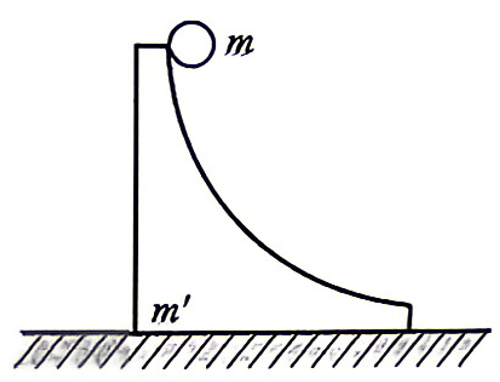
\includegraphics[width=0.3\linewidth]{figure/2-38}
	\caption{习题2-38图}
	\label{fig:2-38}
\end{figure}

\end{enumerate}

\subsection{习题3}
\begin{enumerate}

\item[\textbf{3-10}]
固定在一起的两个同轴均匀圆柱体可绕其光滑的水平对称轴 \(OO'\) 转动。设大小圆柱体的半径分别为 \(R\) 和 \(r\)，质量分别为 \(m'\) 和 \(m\)。绕在两柱体上的细绳分别与物体 \(m_1\) 和 \(m_2\) 相连，\(m_1\) 和 \(m_2\) 则挂在圆柱体的两侧，如习题 3-10 图所示。设 \(R=0.20\,\mathrm{m}\)，\(r=0.10\,\mathrm{m}\)，\(m=4\,\mathrm{kg}\)，\(m'=10\,\mathrm{kg}\)，\(m_1=m_2=2\,\mathrm{kg}\)，且开始时 \(m_1\) 和 \(m_2\) 离地高度均为 \(h=2\,\mathrm{m}\)。


\begin{figure}[H]
	\centering
	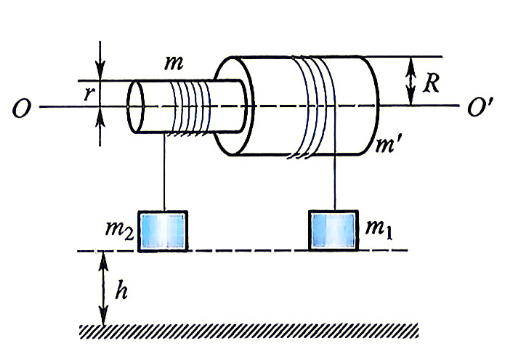
\includegraphics[width=0.3\linewidth]{figure/3-10}
	\caption{习题3-10图}
	\label{fig:3-10}
\end{figure}


\begin{enumerate}
	\item 求柱体转动时的角加速度；
	\item 求两侧细绳的张力；
	\item $m_1$ 和 $m_2$ 哪个先落地？它落地前瞬间的速率为多少？
\end{enumerate}

\item[\textbf{3-11}]
计算如习题 3-11 图所示系统中物体的加速度大小。设滑轮为质量均匀分布的圆柱体，半径为 \(r=0.1\,\mathrm{m}\)，轻绳不可伸长，且与滑轮之间无相对滑动，滑轮轴上摩擦不计，且忽略桌面与物体 \(m_1\) 间的摩擦，已知 \(m_1=50\,\mathrm{kg}\)，\(m_2=200\,\mathrm{kg}\)，滑轮质量 \(m'=15\,\mathrm{kg}\)。

\item[\textbf{3-12}]
如习题 3-12 图所示，一匀质细杆质量为 \(m\)，长为 \(l\)，可绕过一端 \(O\) 的水平光滑固定轴转动，杆从水平位置由静止开始摆下。求：
\begin{enumerate}
	\item 初始时刻的角加速度；
	\item 杆转过 \(\theta\) 角时的角加速度和角速度。
\end{enumerate}

\item[\textbf{3-13}]
如习题 3-13 图所示，一长为 \(1\,\mathrm{m}\) 的均匀直棒可绕其一端与棒垂直的水平光滑固定轴转动，抬起另一端使棒向上与水平面成 \(60^\circ\) 角，然后无初速度地将棒释放，求：
\begin{enumerate}
	\item 放手时棒的角加速度；
	\item 棒转到竖直位置时的角速度。
\end{enumerate}

\item[\textbf{3-14}]
如习题 3-14 图所示，长为 \(L\)、质量为 \(m\) 的均匀细杆静止在水平桌面上，可绕通过左端 \(O\) 点的竖直光滑轴转动。一质量为 \(m_0=m/3\) 的小球以速度 \(v_0\) 垂直击杆于 \(P\) 点，并以速度 \(v=v_0/3\) 弹回。设 \(OP=(3/4)L\)，杆与水平面间的摩擦系数为 \(\mu\)。求：
\begin{enumerate}
	\item 开始转动时的角速度；
	\item 杆所受摩擦力矩的大小；
	\item 杆从开始转动到静止所转过的角度和经历的时间。
\end{enumerate}

\item[\textbf{3-16}]
有一质量为 \(m_1\)、长为 \(l\) 的均匀的细棒 \(OA\)，可绕一端的水平固定轴 \(O\) 自由转动，初始时静止悬挂。一水平运动的质量为 \(m_2\) 的小球，从侧面垂直于棒和轴与棒的另一端 \(A\) 相碰撞，设碰撞时间极短。已知小球在碰撞前后的速度分别为 \(v_1\)、\(v_2\)，方向如习题 3-16 图所示。求：
\begin{enumerate}
	\item 碰撞后瞬间细棒的角速度；
	\item 细棒能够摆动的最大摆角 \(\theta_m\)。
\end{enumerate}

\item[\textbf{3-17}]
如习题 3-17 图所示，一长为 \(l\)、质量为 \(m_1\) 的均质细杆，可绕通过其一端的水平轴 \(O\) 在竖直平面内自由转动，杆从水平位置由静止释放后，与 \(O\) 点正下方静止在光滑水平面上的物体 \(m_2\) 发生碰撞，\(m_2=m_1/3\)。求：
\begin{enumerate}
	\item 杆在转动过程中 \(\theta\) 角加速度 \(\alpha\) 的表达式；
	\item 杆转到竖直位置时的角动量和动能；
	\item 若碰撞是完全弹性的，碰撞后 \(m_2\) 的速度；
	\item 弹簧被压缩的最大长度。
\end{enumerate}


\end{enumerate}

